\documentclass[a4paper,onecolumn]{article}
\usepackage{amsmath, amsthm, graphicx, amssymb, wrapfig, fullpage, subfigure, array}
\usepackage[font=sl, labelfont={sf}, margin=1cm]{caption}
\DeclareMathOperator{\e}{e}
\begin{document}
\setcounter{page}{1}

\title{}
\author{}
\date{}
\maketitle

Consider optimizing on finite time horizon $0$ to $T$
($T\rightarrow\infty$ has similar argument). Action is
$\left\{a\right\} = \left\{a_1, a_2, \cdots, a_T\right\}$,
where unit time represents a tiny physical time $\delta t$.
Unkonwn state indicated by $b_t$.
At time $0$, Monte Carlo sample prior $b_0$ and get $s_1,\cdots,s_N$, and obtain optimal control
\begin{equation*}
    \left\{a^0\right\} = \textrm{argmax}_a \sum_{i=0}^T J(a,s_i)
\end{equation*}
Adopt this control and evolve the true (uncertain) system (e.g. oil
reservoir) for a unit time, obtain
observation $o$.
Assume state $s$ distributed according to $b_0$, we try to find out a
`transport map' $f(s)$ (Tarek 2012, Bayesian Inference with Optimal
Maps) that distributes according to
$$
\propto b_0(s)
\mathbb{P}[o|s,a]\approx \frac{1}{N}\sum_i \mathbb{P}[o|s_i, a]
$$
The map `transports' samples $s_i$ to $f(s_i)$.
At the next time step, we seek to obtain optimal control from an updated
belief
\begin{equation*}
    \left\{a^1\right\} = \textrm{argmax}_a \sum_{i=1}^T J(a,s^1)
\end{equation*}
where
$$
s^1 = f(s_i) \approx s_i + c_i\delta t
$$
Here $\delta t$ is the physical time increment. This is based on the
assumption that information `arrives gradually' (sorry for the poor
wording).
We use adjoint to find $a^1-a^0$'s sensitivity to $c_i$'s.\\
Write the reward for time $0$ to $1$ as $r_0$, and reward from $t$ to
$T$ as $J_t$, then
$J_0 = r_0 + J_1$\\
we have
\begin{equation}
    \left.\frac{\partial r_0}{\partial a} + \frac{\partial J_1}{\partial
	a}\right|_{a^0} = 0
	\label{eq1}
\end{equation}
\begin{equation}
    \left.\frac{\partial J_1}{\partial a}\delta a + \frac{\partial J_1}{\partial
	s} c \delta t \right|_{a^1} = 0
	\label{eq2}
\end{equation}
After approximation
$$
\left.\frac{\partial J_1}{\partial a}\right|_{a^0} \approx
\left.\frac{\partial J_1}{\partial a}\right|_{a^1}
$$
we get
\begin{equation}
    \delta a = \left(\frac{\partial r_0}{\partial
	a}\right)^{-1}\frac{\partial J}{\partial s}c \delta t
\end{equation}
This gives a sequential update formulation of optimal control.
\subsection{Remarks}
1.The key step is to construct the optimal transport map $f$. Tarek
parameters $f$ by parametric chaos on the whole domain of $f$. However, by
noticing $f\approx I + \delta$ for every time increment, I feel there
may be some way to simplify the construction. Not sure how to do it yet.
(requires knowledge of manifold)?
2.The resulting policy is not optimal (the optimal can only be obtained by
backward induction on belief space). Is here any remedy?

\section{History Matching with Ensemble Kalman Filter}
Take incompressible reservoir as an example.
States $x_{0|0}^i = [s_0^i, k_0^i]$ are the $t=0$ 'augmented' samples
consisted of saturation and permeabilities. $y_t$ is the observations
from the true reservoir. The subscript $0|0$ means samples at time $0$
(first 0) based on observations \textbf{at and before} time $0$ (second 0, which
means no observations yet). Superscript index $i=1,\cdots,N$ indicates
the samples.
\subsection{Forecast Step}
Obtain $x_{t|t-1}^i$ from $x_{t-1|t-1}^i$ given control $u_{t-1}$.
The $s_t^i$ part is updated through reservoir simulator
\begin{equation}\begin{split}
    s_{t|t-1}^i &= f(x_{t-1|t-1}^i, u_{t-1})\\
	k_{t|t-1}^i &= k_{t-1|t-1}^i
\end{split}\end{equation}
Forecast observation
\begin{equation}
    y_{t|t-1}^i = g(x^i_{t|t-1},u_t)
\end{equation}
\subsection{Update Step}
\begin{equation}
x_{t|t}^i = x_{t|t-1}^i + Cov[x_{t|t-1}, y_{t|t-1}]
Cov^{-1}[y_{t|t-1},y_{t|t-1}]\left(y_t - y_{t|t-1}^i\right)
\end{equation}

\section{Sequential Optimal Control}
\begin{figure}
\begin{center}
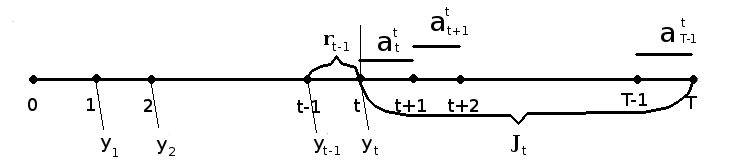
\includegraphics[width=10cm]{time_notation.png}
\end{center}
\end{figure}
Denote $\tilde{J} = \sum_i{J^i}$ as the ensemble objective function.
$\tilde{J}_{t|t}$ indicates the objective function after time $t$ given
the optimal control obtained with the observations $y_1,\cdots,y_t$.\\

\noindent Denote
$$
    a^t = \{a_t^t, a_{t+1}^t, \cdots, a_{T-1}^t\}
$$
as the optimal control starting from time $t$ with observations up to
$y_t$.
$$
    \bar{a}^t = \{a_t^{t-1}, a_{t+1}^{t-1}, \cdots, a_{T-1}^{t-1}\}
$$
as the optimal control starting from time $t$ with observations up to
$y_{t-1}$.

\begin{equation}\begin{split}
    \tilde{J}_{t-1|t-1} &= \sum_i J_{t-1}\left( \{a^{t-1}_{t-1},
	\bar{a}^{t}\}; x^i_{t-1|t-1}\right)\\
	&= \sum_i \left(
	    r_{t-1}(a_{t-1}^{t-1}; x_{t-1|t-1}^i) + J_t\left(
		    \bar{a}^t; x_{t|t-1}^i
		\right)
	\right)
\end{split}\end{equation}
\begin{equation}
    x_{t|t-1}^i = F(x_{t-1|t-1}^i, a_{t-1}^{t-1})
	\label{updatex}
\end{equation}
Eqn\eqref{updatex} can be obtained by EnKF forecast step.
Also,
\begin{equation}
    \tilde{J}_{t|t} = \sum_i J_t\left(
	    a^t; x^i_{t|t}
	\right)
\end{equation}
We have
\begin{equation}\begin{split}
    \frac{d\tilde{J}_{t-1|t-1}}{d a_{t-1}^{t-1}} &= 0\\
	\frac{\partial \tilde{J}_{t-1|t-1}}{\partial \bar{a}^t} &= 0
\end{split}\end{equation}
and
\begin{equation}
    \frac{\partial \tilde{J}_t}{\partial a^t} = 0
\end{equation}
\end{document}








